Global Arrays provide one-sided, noncollective communication operations
that allow to access data in global arrays without cooperation with
the process or processes that hold the referenced data. These processes
do not know what data items in their own memory are being accessed
or updated by remote processes. Moreover, since the GA interface uses
global array indices to reference nonlocal data, the calling process
does not even have to know process ids and location in memory where
the refernenced data resides.

The one-sided operations that Global Arrays provide can be summarized
into three categories: 

\begin{tabular}{|>{\centering}p{4cm}|>{\centering}p{4cm}|}
\hline 
Operation & Process\tabularnewline
\hline
\hline 
Remote blockwise write/read & \texttt{ga\_put, ga\_get}\tabularnewline
\hline 
Remote atomic update & \texttt{ga\_acc, ga\_read\_inc, ga\_scatter\_acc}\tabularnewline
\hline 
Remote elementwise write/read & \texttt{ga\_scatter, ga\_gather}\tabularnewline
\hline
\end{tabular}


\section{Put/Get }

\emph{Put} and \emph{get} are two powerful operations for interprocess
communication, performing remote write and read. Because of their
one-sided nature, they don't need cooperation from the process(es)
that owns the data. The semantics of these operations do not require
the user to specify which remote process or processes own the accessed
portion of a global array. The data is simply accessed as if it were
in shared memory.

Put copies data from the local array to the global array section,
which is
\begin{lyxcode}
\textcolor{green}{n-D}~\textcolor{blue}{Fortran}~subroutine~\href{http://www.emsl.pnl.gov/docs/global/ga_ops.html\#ga_put}{nga\_{}put}(g\_a,~lo,~hi,~buf,~ld)~

\textcolor{green}{2-D}~\textcolor{blue}{Fortran}~subroutine~\href{http://www.emsl.pnl.gov/docs/global/ga_ops.html\#ga_put}{ga\_{}put}(g\_a,~ilo,~ihi,~jlo,~jhi,~buf,~ld)~

\textcolor{blue}{C}~~~~~~~~~~~void~\href{http://www.emsl.pnl.gov/docs/global/c_nga_ops.html\#ga_put}{NGA\_{}Put}(int~g\_a,~int~lo{[}{]},~int~hi{[}{]},~void~{*}buf,~

~~~~~~~~~~~~~~~~~~~~~~~~~int~ld{[}{]})~

\textcolor{blue}{C++}~~~~~~~~~void~GA::GlobalArray::put(int~lo{[}{]},~int~hi{[}{]},~

~~~~~~~~~~~~~~~~~~~~~~~~~void~{*}buf,~int~ld{[}{]})
\end{lyxcode}
All the arguments are provided in one call: \texttt{lo} and \texttt{\noun{hi}}
specify where the data should go in the global array; \texttt{\noun{ld}}
specifies the stride information of the local array \texttt{\noun{buf}}.
The local array should have the same number of dimensions as the global
array; however, it is really required to present the n-dimensional
view of the local memory buffer, that by itself might be one-dimensional.

The operation is transparent to the user, which means the user doesn't
have to worry about where the region defined by \texttt{\noun{lo}}
and \texttt{\noun{hi}} is located. It can be in the memory of one
or many remote processes, owned by the local process, or even mixed
(part of it belongs to remote processes and part of it belongs to
a local process).

\emph{Get} is the reverse operation of \emph{put}. It copies data
from a global array section to the local array. It is
\begin{lyxcode}
\textcolor{green}{n-D}~\textcolor{blue}{Fortran}~subroutine~\href{http://www.emsl.pnl.gov/docs/global/ga_ops.html\#ga_get}{nga\_{}get}(g\_a,~lo,~hi,~buf,~ld)~

\textcolor{green}{2-D}~\textcolor{blue}{Fortran}~subroutine~\href{http://www.emsl.pnl.gov/docs/global/ga_ops.html\#ga_get}{ga\_{}get}(g\_a,~ilo,~ihi,~jlo,~jhi,~buf,~ld)~

\textcolor{blue}{C}~~~~~~~~~~~void~\href{http://www.emsl.pnl.gov/docs/global/c_nga_ops.html\#ga_get}{NGA\_{}get}(int~g\_a,~int~lo{[}{]},~int~hi{[}{]},~

~~~~~~~~~~~~~~~~~~~~~~~~~void~{*}buf,~int~ld{[}{]})~

\textcolor{blue}{C++}~~~~~~~~~void~GA::GlobalArray::get(int~lo{[}{]},~int~hi{[}{]},~

~~~~~~~~~~~~~~~~~~~~~~~~~~void~{*}buf,~int~ld{[}{]})
\end{lyxcode}
Similar to \emph{put}, \texttt{\noun{lo}} and \texttt{\noun{hi}} specify
where the data should come from in the global array, and \texttt{\noun{ld}}
specifies the stride information of the local array \texttt{\noun{buf}}.
The local array is assumed to have the same number of dimensions as
the global array. Users don't need to worry about where the region
defined by \texttt{\noun{lo}} and \texttt{\noun{hi}} is physically
located.

\textit{\underbar{Example}}\textit{\emph{\underbar{:}}}

For a \texttt{\noun{ga\_get}} operation transferring data from the
(11:15,1:5) section of a 2-dimensional 15 x10 global array into a
local buffer 5 x10 array we have: (In Fortran notation)

\begin{center}
\emph{lo}=\{11,1\}, \emph{hi}=\{15,5\}, \emph{ld}=\{10\} 
\par\end{center}

\begin{center}
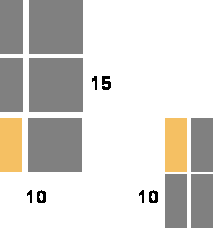
\includegraphics[width=0.4\columnwidth]{GA_get_example}
\par\end{center}


\section{Accumulate and Read-and-increment }

It is often useful in a put operation to combine the data moved to
the target process with the data that resides at that process, rather
then replacing the data there. \emph{Accumulate} and \emph{read\_inc}
perform an \noun{atomic} remote update to a patch (a section of the
global array) in the global array and an element in the global array,
respectively. They don't need the cooperation of the process(es) who
owns the data. Since the operations are atomic, the same portion of
a global array can be referenced by these operations issued by multiple
processes and the GA will assure the correct and consistent result
of the updates.

\emph{Accumulate} combines the data from the local array with data
in the global array section, which is
\begin{lyxcode}
\textcolor{green}{n-D}~\textcolor{blue}{Fortran}~subroutine~\href{http://www.emsl.pnl.gov/docs/global/ga_ops.html\#ga_acc}{nga\_{}acc}(g\_a,~lo,~hi,~buf,~ld,~alpha)~

\textcolor{green}{2-D}~\textcolor{blue}{Fortran}~subroutine~\href{http://www.emsl.pnl.gov/docs/global/ga_ops.html\#ga_acc}{ga\_{}acc}(g\_a,~ilo,~ihi,~jlo,~jhi,~buf,~

~~~~~~~~~~~~~~~~~~~~~~~~~~~~~~ld,~alpha)~

\textcolor{blue}{C}~~~~~~~~~~~void~\href{http://www.emsl.pnl.gov/docs/global/c_nga_ops.html\#ga_acc}{NGA\_{}Acc}(int~g\_a,~int~lo{[}{]},~int~hi{[}{]},~void~{*}buf,~

~~~~~~~~~~~~~~~~~~~~~~~~~int~ld{[}{]},~void~{*}alpha)~

\textcolor{blue}{C++}~~~~~~~~~void~NGA::GlobalArray::acc(int~lo{[}{]},~int~hi{[}{]},~

~~~~~~~~~~~~~~~~~~~~~~~~~~~~~~~~~~~~~~~void~{*}buf,~int~ld{[}{]},~v

~~~~~~~~~~~~~~~~~~~~~~~~~~~~~~~~~~~~~~~oid~{*}alpha)
\end{lyxcode}
The local array is assumed to have the same number of dimensions as
the global array. Users don't need to worry about where the region
defined by lo and hi is physically located. The function performs

\emph{global array section (lo{[}{]}, hi{[}{]})} += \emph{alpha {*}
buf}

Read\_inc remotely updates a particular element in the global array,
which is
\begin{lyxcode}
\textcolor{green}{n-D}~\textcolor{blue}{Fortran}~subroutine~\href{http://www.emsl.pnl.gov/docs/global/ga_ops.html\#ga_read_inc}{nga\_{}read\_{}inc}(g\_a,~subscript,~inc)~

\textcolor{green}{2-D}~\textcolor{blue}{Fortran}~subroutine~\href{http://www.emsl.pnl.gov/docs/global/ga_ops.html\#ga_read_inc}{ga\_{}read\_{}inc}(g\_a,~i,~j,~inc)~

\textcolor{blue}{C}~~~~~~~~~~~long~\href{http://www.emsl.pnl.gov/docs/global/c_nga_ops.html\#ga_read_inc}{NGA\_{}Read\_{}inc}(int~g\_a,~int~subscript{[}{]},~long~inc)~

\textcolor{blue}{C++}~~~~~~~~~long~GA::GlobalArray::readInc(int~subscript{[}{]},~long~inc)
\end{lyxcode}
This function applies to integer arrays only. It atomically reads
and increments an element in an integer array. It performs

\emph{a(subsripts)} += \emph{inc}

and returns the original value (before the update) of \emph{a(subscript)}. 


\section{Scatter/Gather }

\emph{Scatter} and \emph{gather} transfer a specified set of elements
to and from global arrays. They are one-sided: that is they don't
need the cooperation of the process(es) who own the referenced elements
in the global array.

Scatter puts array elements into a global array, which is
\begin{lyxcode}
\textcolor{green}{n-D}~\textcolor{blue}{Fortran}~subroutine~\href{http://www.emsl.pnl.gov/docs/global/ga_ops.html\#ga_scatter}{nga\_{}scatter}(g\_a,~v,~subsarray,~n)~

\textcolor{green}{2-D}~\textcolor{blue}{Fortran}~subroutine~\href{http://www.emsl.pnl.gov/docs/global/ga_ops.html\#ga_scatter}{ga\_{}scatter}(g\_a,~v,~i,~j,~n)~

\textcolor{blue}{C}~~~~~~~~~~~void~\href{http://www.emsl.pnl.gov/docs/global/c_nga_ops.html\#ga_scatter}{NGA\_{}Scatter}(int~g\_a,~void~{*}v,~int~

~~~~~~~~~~~~~~~~~~~~~~~{*}subsarray{[}{]},~int~n)~

\textcolor{blue}{C++~}~~~~~~~~void~GA::GlobalArray::scatter(void~{*}v,~

~~~~~~~~~~~~~~~~~~~~~~~int~{*}subsarray{[}{]},~int~n)
\end{lyxcode}
It performs (in C notation)
\begin{lyxcode}
for(k=0;~k<=~n;~k++)~\{

a{[}subsArray{[}k{]}{[}0{]}{]}{[}subsArray{[}k{]}{[}1{]}{]}{[}subsArray{[}k{]}{[}2{]}{]}...~=~v{[}k{]};~

\}
\end{lyxcode}
\emph{Example}:

Scatter the 5 elements into a 10x10 global array
\begin{lyxcode}
Element~1~v{[}0{]}~=~5~subsArray{[}0{]}{[}0{]}~=~2~

~~~~~~~~~~~~~~~~~~~subsArray{[}0{]}{[}1{]}~=~3~

Element~2~v{[}1{]}~=~3~subsArray{[}1{]}{[}0{]}~=~3~

~~~~~~~~~~~~~~~~~~~subsArray{[}1{]}{[}1{]}~=~4~

Element~3~v{[}2{]}~=~8~subsArray{[}2{]}{[}0{]}~=~8~

~~~~~~~~~~~~~~~~~~~subsArray{[}2{]}{[}1{]}~=~5~

Element~4~v{[}3{]}~=~7~subsArray{[}3{]}{[}0{]}~=~3~

~~~~~~~~~~~~~~~~~~~subsArray{[}3{]}{[}1{]}~=~7~

Element~5~v{[}4{]}~=~2~subsArray{[}4{]}{[}0{]}~=~6~

~~~~~~~~~~~~~~~~~~~subsArray{[}4{]}{[}1{]}~=~3
\end{lyxcode}
After the scatter operation, the five elements would be scattered
into the global array as shown in the following figure. 

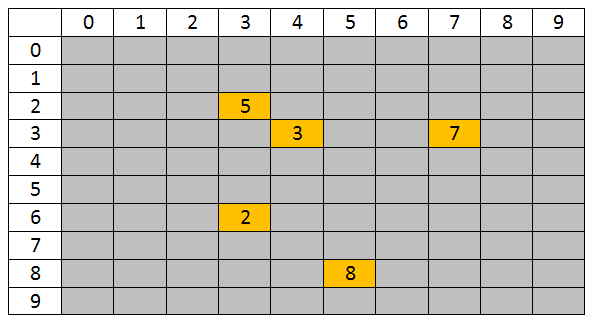
\includegraphics[scale=0.6]{scatter-GA}

\emph{Gather} is the reverse operation of scatter. It gets the array
elements from a global array into a local array.
\begin{lyxcode}
\textcolor{green}{n-D}~\textcolor{blue}{Fortran}~subroutine~\href{http://www.emsl.pnl.gov/docs/global/ga_ops.html\#ga_gather}{nga\_{}gather}(g\_a,~v,~subsarray,~n)~

\textcolor{green}{2-D}~\textcolor{blue}{Fortran}~subroutine~\href{http://www.emsl.pnl.gov/docs/global/ga_ops.html\#ga_gather}{ga\_{}gather}ga\_gather(g\_a,~v,~i,~j,~n)~

\textcolor{blue}{C}~~~~~~~~~~~void~\href{http://www.emsl.pnl.gov/docs/global/c_nga_ops.html\#ga_gather}{NGA\_{}Gather}(int~g\_a,~void~{*}v,~

~~~~~~~~~~~~~~~~~~~~~~~~~~~~~int~{*}subsarray{[}{]},~int~n)~

\textcolor{blue}{C++}~~~~~~~~~void~GA::GlobalArray::gather(void~{*}v,~int~

~~~~~~~~~~~~~~~~~~~~~~~~~~~~~{*}subsarray{[}{]},~int~n)
\end{lyxcode}
It performs (in C notation)
\begin{lyxcode}
for(k=0;~k<=~n;~k++)\{~

~~~~~v{[}k{]}~=~a{[}subsArray{[}k{]}{[}0{]}{]}{[}subsArray{[}k{]}{[}1{]}{]}{[}subsArray{[}k{]}{[}2{]}{]}...;~

\}~
\end{lyxcode}

\section{Periodic Interfaces }

Periodic interfaces to the one-sided operations have been added to
Global Arrays in version 3.1 to support some computational fluid dynamics
problems on multidimensional grids. They provide an index translation
layer that allows you to use put, get, and accumulate operations,
possibly extending beyond the boundaries of a global array. The references
that are outside of the boundaries are wrapped up inside the global
array. To better illustrate these operations, look at the following
example:

\emph{Example}: 

Assume a two dimensional global array g\_a with dimensions 5 X 5.

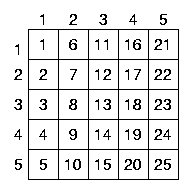
\includegraphics[width=7cm]{periodic1}

To access a patch {[}2:4,-1:3{]}, one can assume that the array is
wrapped over in the second dimension, as shown in the following figure 

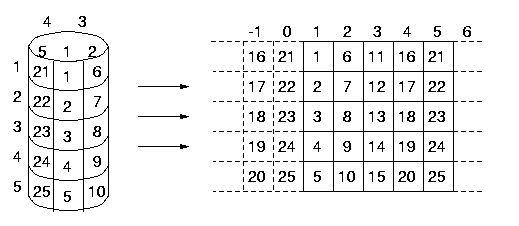
\includegraphics[scale=0.7]{periodic2}

Therefore the patch {[}2:4, -1:3{]} is
\begin{lyxcode}
17~22~2~7~12~

18~23~3~8~13~

19~24~4~9~14
\end{lyxcode}
Periodic operations extend the boudary of each dimension in two directions,
toward the lower bound and toward the upper bound. For any dimension
with lo(i) to hi(i), where 1 < i < ndim, it extends the range from 
\begin{lyxcode}
{[}lo(i)~:~hi(i){]}~
\end{lyxcode}
to 
\begin{lyxcode}
{[}(lo(i)-1-(hi(i)-lo(i)+1))~:~(lo(i)-1){]},~{[}lo(i)~:~hi(i){]},~
\end{lyxcode}
and 
\begin{lyxcode}
{[}(hi(i)+1)~:~(hi(i)+1+(hi(i)-lo(i)+1)){]},~
\end{lyxcode}
or 
\begin{lyxcode}
{[}(lo(i)-1-(hi(i)-lo(i)+1))~:~(hi(i)+1+(hi(i)-lo(i)+1)){]}.
\end{lyxcode}
Even though the patch spans in a much large range, the length must
always be less, or equal to (hi(i)-lo(i)+1)).

\emph{Example}: For a 2 x 2 array as shown in the following figure,
where the dimensions are {[}1:2, 1:2{]}, periodic operations would
look at the range of each of the dimensions as {[}-1:4, -1:4{]}.

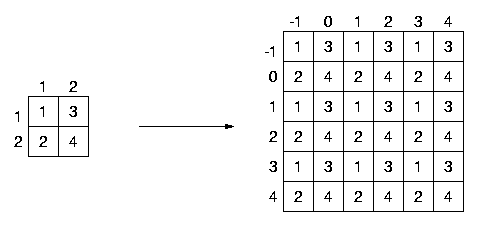
\includegraphics[scale=0.7]{periodic3}

Current version of GA supports three periodic operations. They are
\begin{itemize}
\item periodic get, 
\item periodic put, and 
\item periodic accumulate
\end{itemize}
\emph{Periodic Get }copies data from a global array section to a local
array, which is almost the same as regular get, except the indices
of the patch can be outside the boundaries of each dimension.
\begin{lyxcode}
\textcolor{blue}{Fortran}~subroutine~\href{http://www.emsl.pnl.gov/docs/global/ga_ops.html\#ga_periodic_get}{nga\_{}periodic\_{}get}(g\_a,~lo,~hi,~buf,~ld)~

\textcolor{blue}{C}~~~~~~~void~\href{http://www.emsl.pnl.gov/docs/global/c_nga_ops.html\#ga_periodic_get}{NGA\_{}Periodic\_{}get}(int~g\_a,~int~lo{[}{]},~int~hi{[}{]},~

~~~~~~~~~~~~~void~{*}buf,~int~ld{[}{]})~

\textcolor{blue}{C++}~~~~~void~GA::GlobalArray::periodicGet(int~lo{[}{]},~

~~~~~~~~~~~~~int~hi{[}{]},~void~{*}buf,~int~ld{[}{]})
\end{lyxcode}
Similar to regular \emph{get}, \texttt{\noun{lo}} and \texttt{\noun{hi}}
specify where the data should come from in the global array, and \texttt{\noun{ld}}
specifies the stride information of the local array \texttt{\noun{buf}}.

\emph{Example}: Let us look at the first example in this section.
It is 5 x 5 two dimensional global array. Assume that the local buffer
is an 4x3 array. 

Also assume that
\begin{lyxcode}
1o{[}0{]}~=~-1,~hi{[}0{]}~=~2,~

lo{[}1{]}~=~4,~hi{[}1{]}~=~6,~and~

ld{[}0{]}~=~4.
\end{lyxcode}
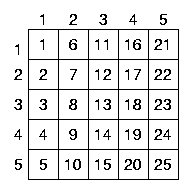
\includegraphics[width=7cm]{periodic1}

The local buffer \texttt{\noun{buf}} is
\begin{lyxcode}
19~~~~24~~~~4~

20~~~~25~~~~5~~

16~~~~21~~~~1~

17~~~~22~~~~2~
\end{lyxcode}
Periodic Put is the reverse operations of Periodic Get. It copies
data from the local array to the global array section, which is
\begin{lyxcode}
\textcolor{blue}{Fortran}~subroutine~\href{http://www.emsl.pnl.gov/docs/global/ga_ops.html\#ga_periodic_put}{nga\_{}periodic\_{}put}(g\_a,~lo,~hi,~buf,~ld)~

\textcolor{blue}{C}~~~~~~~void~\href{http://www.emsl.pnl.gov/docs/global/c_nga_ops.html\#ga_periodic_put}{NGA\_{}Periodic\_{}put}(int~g\_a,~int~lo{[}{]},~int~hi{[}{]},~

~~~~~~~~~~~~~void~{*}buf,~int~ld{[}{]})~

\textcolor{blue}{C++}~~~~~void~GA::GlobalArray::periodicPut(int~lo{[}{]},~

~~~~~~~~~~~~~int~hi{[}{]},~void~{*}buf,~int~ld{[}{]})
\end{lyxcode}
Similar to regular\emph{ put}, \texttt{\noun{lo}} and \texttt{\noun{hi}}
specify where the data should go in the global array; \texttt{\noun{ld}}
specifies the stride information of the local array \texttt{\noun{buf}}.

\emph{Periodic Put/Get} (also include the \emph{Accumulate}, which
will be discussed later in this section) divide the patch into several
smaller patches. For those smaller patches that are outside the global
aray, adjust the indices so that they rotate back to the original
array. After that call the regular \emph{Put/Get/Accumulate}, for
each patch, to complete the operations.

\emph{Example}: Look at the example for periodic get. Because it is
a 5 x 5 global array, the valid indices for each dimension are
\begin{lyxcode}
dimension~0:~{[}1~:~5{]}~

dimension~1:~{[}1~:~5{]}
\end{lyxcode}
The specified lo and hi are apparently out of the range of each dimension:
\begin{lyxcode}
dimemsion~0:~{[}-1~:~2{]}~-{}->~{[}-1~:~0{]}~-{}-~wrap~back~-{}->~{[}4~:~5{]}~{[}~1~:~2{]}~ok

dimension~1:~{[}~4~:~6{]}~-{}->~{[}~4~:~5{]}~ok~{[}~6~:~6{]}~-{}-~wrap~back~-{}->~{[}1~:~1{]}
\end{lyxcode}
Hence, there will be four smaller patches after the adjustment. They
are
\begin{lyxcode}
patch~0:~{[}4~:~5,~4~:~5{]}~

patch~1:~{[}4~:~5,~1~:~1{]}~

patch~2:~{[}1~:~2,~4~:~5{]}~

patch~3:~{[}1~:~2,~1~:~1{]}
\end{lyxcode}
as shown in the following figure

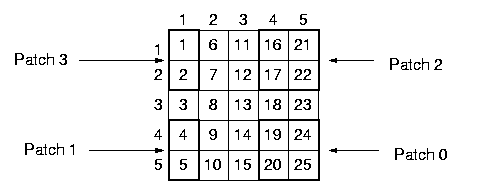
\includegraphics[width=0.7\paperwidth]{periodic4}

Of course the destination addresses of each samller patch in the local
buffer also need to be calculated.

Similar to regular \emph{Accumulate, Periodic Accumulate} combines
the data from the local array with data in the global array section,
which is
\begin{lyxcode}
\textcolor{blue}{Fortran}~subroutine~\href{http://www.emsl.pnl.gov/docs/global/ga_ops.html\#ga_periodic_acc}{nga\_{}periodic\_{}acc}(g\_a,~lo,~hi,~buf,~ld,~alpha)~

\textcolor{blue}{C}~~~~~~~void~\href{http://www.emsl.pnl.gov/docs/global/c_nga_ops.html\#ga_periodic_acc}{NGA\_{}Periodic\_{}acc}(int~g\_a,~int~lo{[}{]},~int~hi{[}{]},~

~~~~~~~~~~~~~~~~~~~void~{*}buf,~int~ld{[}{]},~void~{*}alpha)~

\textcolor{blue}{C++~}~~~~void~GA::GlobalArray::periodicAcc(int~lo{[}{]},~int~hi{[}{]},~

~~~~~~~~~~~~~~~~~~~void~{*}buf,~int~ld{[}{]},~void~{*}alpha)
\end{lyxcode}
The local array is assumed to have the same number of dimensions as
the global array. Users don't need to worry about where the region
defined by \texttt{\noun{lo}} and \texttt{\noun{hi}} is physically
located. The function performs

\emph{global array section (lo{[}{]}, hi{[}{]}) += alpha {*} buf}

\emph{Example}: Let us look at the same example as above. There is
a 5 x 5 two dimensional global array. Assume that the local buffer
is an 4x3 array. 

Also assume that
\begin{lyxcode}
1o{[}0{]}~=~-1,~hi{[}0{]}~=~2,~

lo{[}1{]}~=~4,~hi{[}1{]}~=~6,~and~

ld{[}0{]}~=~4.
\end{lyxcode}
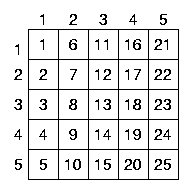
\includegraphics[width=7cm]{periodic1}

The local buffer buf is
\begin{lyxcode}
1~~5~~9~

4~~6~~5~

3~~2~~1~

7~~8~~2
\end{lyxcode}
and the \texttt{\noun{alpha = 2}}.

After the Periodic Accumulate operation, the global array will be

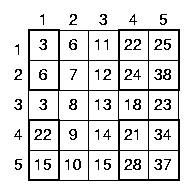
\includegraphics[width=7cm]{periodic5}


\section{Non-blocking operations}

The non-blocking operations (get/put/accumulate) are derived from
the blocking interface by adding a handle argument that identifies
an instance of the non-blocking request. Nonblocking operations initiate
a communication call and then return control to the application. A
return from a nonblocking operation call indicates a mere initiation
of the data transfer process and the operation can be completed locally
by making a call to the wait (e.g. nga\_nbwait) routine.

The wait function completes a non-blocking one-sided operation locally.
Waiting on a nonblocking put or an accumulate operation assures that
data was injected into the network and the user buffer can be now
be reused. Completing a get operation assures data has arrived into
the user memory and is ready for use. Wait operation ensures only
local completion. Unlike their blocking counterparts, the nonblocking
operations are not ordered with respect to the destination. Performance
being one reason, the other reason is that by ensuring ordering we
incur additional and possibly unnecessary overhead on applications
that do not require their operations to be ordered. For cases where
ordering is necessary, it can be done by calling a fence operation.
The fence operation is provided to the user to confirm remote completion
if needed.

\begin{tabular}{|>{\raggedright}p{13cm}|}
\hline 
\emph{Example}: Let us take a simple case for illustration. Say, there
are two global arrays i.e. one array stores pressure and the other
stores temperature. If there are two computation phases (first phase
computes pressure and second phase computes temperature), then we
can overlap communication with computation, thus hiding latency.\tabularnewline
\hline 
\begin{lyxcode}
.~.~.~.~.~.~.~.~.~

nga\_get~(get\_pressure\_array)

nga\_nbget(initiates~data~transfer~to~get~temperature\_array,~

~~~~~and~returns~immediately)

compute\_pressure()~/{*}~hiding~latency~-~communication~

~~~~~is~overlapped~with~computation~{*}/

nga\_nbwait(temperature\_array~-~completes~data~transfer)

compute\_temperature()~

.~.~.~.~.~.~.~.
\end{lyxcode}
\tabularnewline
\hline
\end{tabular}

The non-blocking APIs are derived from the blocking interface by adding
a handle argument that identifies an instance of the non-blocking
request.
\begin{lyxcode}
\textcolor{green}{n-D}~\textcolor{blue}{Fortran}~subroutine~\href{http://www.emsl.pnl.gov/docs/global/ga_ops.html\#nga_nbput}{nga\_{}nbput}(g\_a,~lo,~hi,~buf,~ld,~nbhandle)~

\textcolor{green}{n-D}~Fortran~subroutine~\href{http://www.emsl.pnl.gov/docs/global/ga_ops.html\#nga_nbget}{nga\_{}nbget}(g\_a,~lo,~hi,~buf,~ld,~nbhandle)~

\textcolor{green}{n-D}~\textcolor{blue}{Fortran}~subroutine~\href{http://www.emsl.pnl.gov/docs/global/ga_ops.html\#nga_nbacc}{nga\_{}nbacc}(g\_a,~lo,~hi,~buf,~ld,~alpha,~

~~~~~~~~~~~~~~~~~~~~~nbhandle)~

\textcolor{green}{n-D}~\textcolor{blue}{Fortran}~subroutine~\href{http://www.emsl.pnl.gov/docs/global/ga_ops.html\#nga_nbwait}{nga\_{}nbwait}(nbhandle)

\textcolor{green}{2-D}~\textcolor{blue}{Fortran}~subroutine~\href{http://www.emsl.pnl.gov/docs/global/ga_ops.html\#ga_nbput}{ga\_{}nbput}(g\_a,~ilo,~ihi,~jlo,~jhi,~buf,

~~~~~~~~~~~~~~~~~~~~~ld,~nbhandle)~

\textcolor{green}{2-D}~\textcolor{blue}{Fortran}~subroutine~\href{http://www.emsl.pnl.gov/docs/global/ga_ops.html\#ga_nbget}{ga\_{}nbget}(g\_a,~ilo,~ihi,~jlo,~jhi,~buf,~

~~~~~~~~~~~~ld,~nbhandle)~

\textcolor{green}{2-D}~\textcolor{blue}{Fortran}~subroutine~\href{http://www.emsl.pnl.gov/docs/global/ga_ops.html\#ga_nbacc}{ga\_{}nbacc}(g\_a,~ilo,~ihi,~jlo,~jhi,~buf,~

~~~~~~~~~~~~ld,~alpha,~nbhandle)~

\textcolor{green}{2-D}~\textcolor{blue}{Fortran}~subroutine~\href{http://www.emsl.pnl.gov/docs/global/ga_ops.html\#ga_nbwait}{ga\_{}nbwait}(nbhandle)

\textcolor{blue}{C}~~~~~~~~~~~void~\href{http://www.emsl.pnl.gov/docs/global/c_nga_ops.html\#ga_nbput}{NGA\_{}NbPut}(int~g\_a,~int~lo{[}{]},~int~hi{[}{]},~

~~~~~~~~~~~~~~~~~~~~~void~{*}buf,~int~ld{[}{]},~ga\_nbhdl\_t{*}~nbhandle)~

\textcolor{blue}{C}~~~~~~~~~~~void~\href{http://www.emsl.pnl.gov/docs/global/c_nga_ops.html\#ga_nbget}{NGA\_{}NbGet}(int~g\_a,~int~lo{[}{]},~int~hi{[}{]},~

~~~~~~~~~~~~~~~~~~~~~void~{*}buf,~int~ld{[}{]},~ga\_nbhdl\_t{*}~nbhandle)~

\textcolor{blue}{C}~~~~~~~~~~~void~\href{http://www.emsl.pnl.gov/docs/global/c_nga_ops.html\#ga_nbacc}{NGA\_{}NbAcc}(int~g\_a,~int~lo{[}{]},~int~hi{[}{]},~

~~~~~~~~~~~~~~~~~~~~~void~{*}buf,~int~ld{[}{]},~void~{*}alpha,~

~~~~~~~~~~~~~~~~~~~~~ga\_nbhdl\_t{*}~nbhandle)~

\textcolor{blue}{C}~~~~~~~~~~~int~\href{http://www.emsl.pnl.gov/docs/global/c_nga_ops.html\#ga_nbwait}{NGA\_{}NbWait}(ga\_nbhdl\_t{*}~nbhandle)

\textcolor{blue}{C++}~~~~~~~~~void~GA::GlobalArray::nbPut(int~lo{[}{]},~int~hi{[}{]},~

~~~~~~~~~~~~~~~~~~~~~~~~~~~~~~~~~~~~~~~~void~{*}buf,~

~~~~~~~~~~~~~int~ld{[}{]},~ga\_nbhdl\_t{*}~nbhandle)~

\textcolor{blue}{C++}~~~~~~~~~void~GA::GlobalArray::nbGet(int~lo{[}{]},~int~hi{[}{]},~

~~~~~~~~~~~~~~~~~~~~~~~~~~~~~~~~~~~~~~~void~{*}buf,~

~~~~~~~~~~~~~int~ld{[}{]},~ga\_nbhdl\_t{*}~nbhandle)~

\textcolor{blue}{C++}~~~~~~~~~void~GA::GlobalArray::nbAcc(int~lo{[}{]},~int~hi{[}{]},~

~~~~~~~~~~~~~~~~~~~~~~~~~~~~~~~~~~~~~~~void~{*}buf,~

~~~~~~~~~~~~~int~ld{[}{]},~void~{*}alpha,~ga\_nbhdl\_t{*}~nbhandle)~

\textcolor{blue}{C++}~~~~~~~~~int~GA::GlobalArray::NbWait(ga\_nbhdl\_t{*}~nbhandle)
\end{lyxcode}

